\documentclass[xcolor=dvipsnames]{beamer}
%
% Choose how your presentation looks.
%
% For more themes, color themes and font themes, see:
% http://deic.uab.es/~iblanes/beamer_gallery/index_by_theme.html
%

\usetheme{Dresden}      % or try Darmstadt, Madrid, Warsaw, Goettingen...
\usecolortheme{beaver}  % or try albatross, beaver, crane, ... seahorse
\usefonttheme{default}  % or try serif, structurebold, ...
\setbeamertemplate{navigation symbols}{}
\setbeamertemplate{section}[numbered]

% Changing the color of itemize item in beamer
\setbeamercolor{enumerate item}{fg=darkred}
\setbeamercolor{itemize item}{fg=darkred}
\setbeamercolor{itemize subitem}{fg=darkred}
\setbeamercolor{description item}{fg=darkred}


\usepackage[english]{babel}
\usepackage[utf8x]{inputenc}
\usepackage{multicol}
\usepackage{amsmath,amssymb,amsthm}
\usepackage{amsfonts}
\usepackage{pgfpages}
\usepackage{listings}
% all keywords defined
\lstdefinelanguage[MyLaTeX]{TeX}[LaTeX]{TeX}%
  % TeX commands
  {moretexcs={enquote,includegraphics,%
    part,chapter,section,subsection,paragraph,subparagraph%
    tableofcontents,listoffigures,listoftables,maketitle,%
    subsection,subsubsection,paragraph,autoref,it,%
    textcolor,colorbox,xdefinecolor,colorlet,foreach,%
    rowcolors,rowcolor,lstdefinestyle,lstset,KOMAoptions,%
    setkomavar,setkomavar*,opening,closing,encl,%
    lehead,cehead,rehead,lefoot,cefoot,refoot,%
    lohead,cohead,rohead,lofoot,cofoot,rofoot,%
    ohead,chead,ihead,ofoot,cfoot,ifoot,%
    areaset,color,%
    automark,manualmark,markright,markboth,%
    tableofcontents,url,clearscrheadfoot,pagemark,headmark,%
    setheadtopline,setkomafont,setheadsepline,setfootsepline,%
    setfootbotline,chaptermark,thesection,thechapter,%
    thesubsection,subtitle,inst,section*,subsection*,institute,%
    chapter*,part*,%
    qedhere,usetheme,useinnertheme,useoutertheme,usecolortheme,%
    ,uncover,only,alert,invisible,onslide,mode,mode*,usetikzlibrary,%
    draw,filldraw,path,node,usefonttheme,setbeamertemplate,%
    declaretheorem,FiveFlowerOpen,%
    frontmatter,mainmatter,appendix,backmatter,%
    operatorname, titlegraphic, AtBeginSection},%
  % LaTeX environments
  morekeywords={[2]lstlisting,document,letter,center,flushleft,%
    flushright,align,itemize,enumerate,description,tabular,%
    titlepage,figure,table,frame,tikzpicture,quote,quotation,verse, 
    columns, column, theorem, block},%
  % other things (like packages) to highlight
  morekeywords={[3]listings,textcomp,courier,xcolor,scrartcl,%
    scrlttr2,inputenc,babel,pause,%
    fontenc,lmodern,mathptmx,%
    helvet,geometry,scrpage2,scrreprt,scrbook,%
    article,report,book,hyperref,%
    csquotes,amsmath,amssymb,la,beamer,beamerarticle,%
    tikz,amsthm,thmtools},
  alsoletter={0123456789*},
  morekeywords={[4]Optionen},
  alsoletter={0123456789*}
  }%

%% ------ Colors ------
\definecolor{CadetBlue}{rgb}{.37, .62, .63}
\definecolor{Gray}{rgb}{.70, .70, .70}
\colorlet{maincolor}{orange}
\colorlet{alertedcolor}{red}
\colorlet{examplecolor}{green!50!black}
\colorlet{texicon}{examplecolor}
\colorlet{pdficon}{maincolor}
\colorlet{auxicon}{-examplecolor}
\colorlet{logicon}{black}
\colorlet{bblicon}{-maincolor}
\colorlet{bibicon}{alertedcolor}
\colorlet{texcs}{violet!70}


%% ----- Listings -----
\lstset{ %
  basicstyle=\footnotesize\fontfamily{pcr}\selectfont,        % the size of the fonts that are used for the code
  backgroundcolor=\color{maincolor!10},             % select a background color
  breakatwhitespace=false,         % sets if automatic breaks should only happen at whitespace
  breaklines=true,                 % sets automatic line breaking
  commentstyle=\ttfamily\color{Green}\fontfamily{pcr}\selectfont, % comment style
  deletekeywords={...},            % if you want to delete keywords from the given language
  extendedchars=true,              % lets you use non-ASCII characters; for 8-bits encodings only, does not work with UTF-8
  frame=lines,                     % adds a frame around the code
  keepspaces=true,                 % keeps spaces in text, useful for keeping indentation of code (possibly needs columns=flexible)
  keywordstyle=\ttfamily\color{Blue}\fontfamily{pcr}\selectfont\bfseries, % keyword style
  keywordstyle={[2]\ttfamily\color{Emerald}\fontfamily{pcr}\selectfont\bfseries},
  keywordstyle={[3]\ttfamily\color{Orange}\fontfamily{pcr}\selectfont\bfseries},
  keywordstyle={[4]\ttfamily\color{red}\fontfamily{pcr}\selectfont\bfseries},
  identifierstyle=\ttfamily\color{black}\fontfamily{pcr}\selectfont,
  numbers=left,                    % where to put the line-numbers; possible values are (none, left, right)
  numbersep=5pt,                   % how far the line-numbers are from the code
  numberstyle=\tiny\color{Gray}\fontfamily{pcr}\selectfont, % the style that is used for the line-numbers
  rulecolor=\color{black},         % if not set, the frame-color may be changed on line-breaks within not-black text (e.g. comments (green here))
  showspaces=false,                % show spaces everywhere adding particular underscores; it overrides 'showstringspaces'
  showstringspaces=false,          % underline spaces within strings only
  showtabs=false,                  % show tabs within strings adding particular underscores
  stepnumber=1,                    % the step between two line-numbers. If it's 1, each line will be numbered
  stringstyle=\ttfamily\color{Gray}\fontfamily{pcr}\selectfont,     % string literal style
  tabsize=2,                    % sets default tabsize to 2 spaces
  escapeinside={(*@}{@*)},
}

\lstdefinelanguage{pseudocode}{
  keywordstyle=\ttfamily\textbf{\fontfamily{pcr}}\selectfont,
  identifierstyle=\ttfamily\color{black}\fontfamily{pcr}\selectfont,
  commentstyle=\color{PseudocodeComment}\fontfamily{pcr}\selectfont,
  stringstyle=\ttfamily\fontfamily{pcr}\color{PseudocodeString}\selectfont,
  %morekeywords={documentclass, usepackage, begin, end, frame},
  morecomment=[l]{//},
  morecomment=[s]{/*}{*/},
  morestring=[b]",
  sensitive=false,
  showstringspaces=false,
  rulecolor=\color{Gray},
  escapechar=@,
}

\lstset{
  literate={ö}{{\"o}}1
           {Ö}{{\"O}}1
           {ä}{{\"a}}1
           {Ä}{{\"A}}1
           {ü}{{\"u}}1
           {Ü}{{\"U}}1
           {ß}{{\ss}}1
}


\usepackage{xcolor}
\usepackage{framed}

\usepackage{pgfplots}
\usepackage{tikz}
\usetikzlibrary{positioning,%
  fit,%
  arrows,%
  automata,%
  trees,%
  intersections,%
  mindmap,%
  shapes.geometric,%
  shapes.arrows,%
  decorations,%
  decorations.pathmorphing,%
  decorations.pathreplacing,%
  matrix,%
  chains,%
  scopes,%
  circuits,%
  circuits.ee.IEC,%
  calc,%
  fadings,%
  lindenmayersystems,%
  decorations.markings,%
  shadows,%
  svg.path,%
  scopes,
  shapes,
  decorations.shapes,
  decorations.fractals,
  decorations.markings,
  shadows
}

% those small pics from a sheet
\newcommand*{\icon}[2][2]{%
  \tikz\draw[very thick, line join=round]
    (-.5,.5) -- ++(.7,0) -- ++(.3,-.3) --
    ++(-.3,0) -- ++(0,.3) -- ++(.3,-.3) -- ++(0,-.4)
    \foreach \x in {1,...,#1} {
      -- ++(0,-.2)
    }
    -- ++(-1,0) -- cycle
    (-.5,.2) node[fill, text=white,
      inner sep=2pt, minimum width=8mm, anchor=center] {#2}
    ++ (.1,-.3) -- ++(.8,0) \foreach \x in {1,...,#1} {
      -- ++(0,-.1) -- ++(-.8,0) -- ++(0,-.1) -- ++(.8,0)
    };
}

% Color Definition


\lstdefinelanguage{BibTeX}
{keywords={%
  @article,@book,@collectedbook,@conference,@electronic,@ieeetranbstctl,%
  @inbook,@incollectedbook,@incollection,@injournal,@inproceedings,%
  @manual,@mastersthesis,@misc,@patent,@periodical,@phdthesis,@preamble,%
  @proceedings,@standard,@string,@techreport,@unpublished%
  },
comment=[l][\itshape]{@comment},
morekeywords={[2]author,title,year,publisher,editor,booktitle,journal,series,volume,number,pages,institution,note,howpublished},
 }

\newenvironment{mybib}{%
  \begin{thebibliography}{10}
}{%
  \end{thebibliography}
}

% needed in table
\usepackage{pifont}
\newcommand{\goodmark}{\textcolor{green!50!black}{\Pisymbol{pzd}{52}}}
\newcommand{\badmark}{\textcolor{red}{\Pisymbol{pzd}{56}}}


\lstset{language=[MyLaTeX]{TeX}}
\lstset{columns=fixed}
\lstMakeShortInline[columns=fixed]|

\setbeamertemplate{blocks}[rounded][shadow=true]
\setbeamercolor{block title}{fg=black ,bg=gray!20!bg}
\setbeamercolor{block body}{fg=black ,bg=gray!5!bg}


\newcommand{\tikzexample}[1]{\begin{center}\colorbox{red!5}{#1}\end{center}}

\title{Zeichnen mit TikZ}
\author{Dennis Labitzke}
%\institute{MetaNook}
\date{11.11.2016 -- MetaNook}

\setbeamerfont{frametitle}{size=\small}
\setbeamerfont{framesubtitle}{size=\tiny}

\newsavebox{\mycandle}
\savebox{\mycandle}{ 

\begin{tikzpicture}[scale=.1]
\shade[top color=yellow,bottom color=red] (0,0) .. controls (1,.2) and (1,.5) .. (0,2) .. controls (-1,.5)  and  (-1,.2) .. (0,0);
\fill[yellow!90!black] (.8,0) rectangle (-.8,-5); 
\end{tikzpicture} }
\tikzset{
  paint/.style={draw=#1!50!black, fill=#1!50},
  my star/.style={decorate,decoration={shape backgrounds,shape=star},
                  star points=#1}
} 

\begin{document}

\begin{frame}
  \titlepage
\end{frame}


\begin{frame}{Überblick}
\tableofcontents
\end{frame}


\section{Einführung}
\begin{frame}{Was ist TikZ?}
    \begin{itemize}
        \item
            TikZ ist kein Zeichenprogramm
        \item
            TikZ ist Makropaket zum Zeichnen von Grafiken mit \LaTeX
        \item
            TikZ verfügt über eine sehr ausführliche und gute Anleitung
    \end{itemize}
\end{frame}


\begin{frame}{Ein erstes Beispiel}
    \tikzexample{
        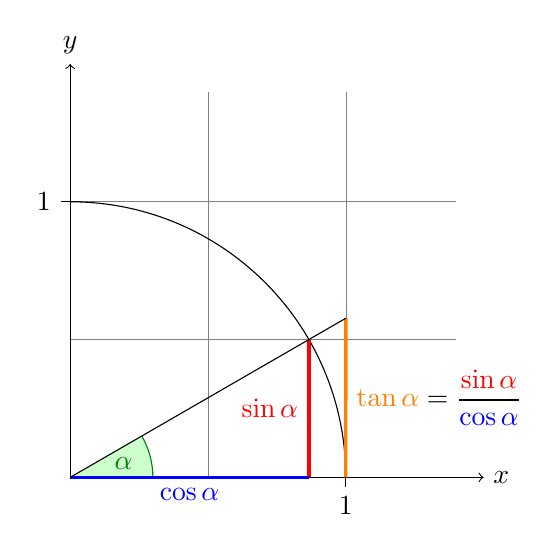
\begin{tikzpicture}[scale=3.5]
            \draw [step=.5cm,gray,very thin] (0,0) grid (1.4,1.4);
            \draw (1,0) arc (0:90:1cm);
            \draw[->] (0,0) -- (1.5,0) node[right] {$x$};
            \draw[->] (0,0) -- (0,1.5) node[above] {$y$};
            \draw (1,1pt) -- (1,-1pt) node[below] {$1$};
            \draw (1pt,1) -- (-1pt,1) node[left] {$1$};
            \filldraw[fill=green!20,draw=green!50!black]
                (0,0) -- (3mm,0pt) arc (0:30:3mm);
            \draw (15:2mm) node[green!50!black] {$\alpha$};
            \draw[very thick,red]
                (30:1cm) -- node[left]
                    {$\sin \alpha$} (30:1cm |- 0,0);
            \draw[very thick,blue]
                (0,0) -- node[below]
                    {$\cos \alpha$} (30:1cm |- 0,0);
            \path [name path=upward line]
                (1,0) -- (1,1);
            \path [name path=sloped line]
                (0,0) -- (30:1.5cm);
            \draw [name intersections=
                {of=upward line and sloped line, by=tan}]
                    [very thick,orange] (1,0) -- node [right]
                        {$\displaystyle \tan \alpha \color{black}=
                            \frac{{\color{red}\sin \alpha}}
                            {\color{blue}\cos \alpha}$} (tan);
            \draw (0,0) -- (tan);
        \end{tikzpicture}
    }
\end{frame}


\subsection{Verwendung}
\begin{frame}[fragile]{TikZ verwenden}
    \tikzexample{
        Wir beginnen mit
        \begin{tikzpicture}
            \draw (0,1) -- (0,0) -- (1,0);
        \end{tikzpicture}
        einem Winkel.
    }

    \begin{lstlisting}[gobble=8]
        \documentclass{scrartcl}
        \usepackage{tikz}
        \begin{document}
            Wir beginnen mit
            \begin{tikzpicture}
                \draw (0,1) -- (0,0) -- (1,0);
            \end{tikzpicture}
            einem Winkel.
        \end{document}
    \end{lstlisting}
\end{frame}


\subsection{Pfade}
\begin{frame}[fragile]{Pfade}
    \begin{itemize}
        \item
            Ein Pfad ist eine Folge von Koordinaten
            \begin{itemize}
                \item
                    Links unten ist der Ursprung $(0{,}0)$
                \item
                    Erste Koordinate: $x$-Richtung
                \item
                    Zweite Koordinate: $y$-Richtung
            \end{itemize}
        \item
            Linien zeichnen mit \lstinline{--}
        \item
            Relative Koordinaten beginnen mit  \lstinline{++}
    \end{itemize}
    
    \tikzexample{
        \begin{tikzpicture}
            \draw
                (0,0) -- ++ (1,0) ++ (0,1) -- ++ (-1,0)
                (2,0) rectangle (3,1);
        \end{tikzpicture}
    }
    
    \begin{lstlisting}[gobble=8]
        \begin{tikzpicture}
            \draw (0,0) -- ++ (1,0) ++ (0,1) -- ++ (-1,0);
            \draw (2,0) rectangle (3,1);
        \end{tikzpicture}
    \end{lstlisting}
\end{frame}


\begin{frame}[fragile]{Gitterpfade}
    \tikzexample{
        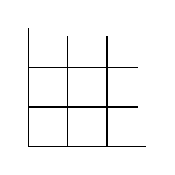
\begin{tikzpicture}
            \draw [step=0.5cm] (0,0) grid (1.4,1.4);
            \draw (0,1.5) -- (0,0) -- (1.5,0);
        \end{tikzpicture}
    }
    
    \begin{lstlisting}[gobble=8]
        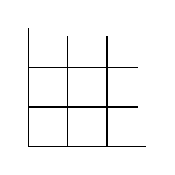
\begin{tikzpicture}
            \draw [step=0.5cm]
                (0,0) grid (1.4,1.4);
            \draw (0,1.5) -- (0,0) -- (1.5,0);
        \end{tikzpicture}
    \end{lstlisting}
\end{frame}


\begin{frame}[fragile]{Skalierung}
    \tikzexample{
        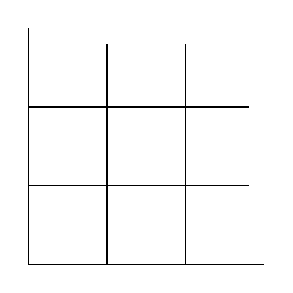
\begin{tikzpicture}[scale=2]
            \draw [step=0.5cm] (0,0) grid (1.4,1.4);
            \draw (0,1.5) -- (0,0) -- (1.5,0);
        \end{tikzpicture}
    }
    
    \begin{lstlisting}[gobble=8]
        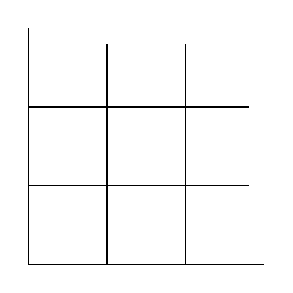
\begin{tikzpicture}[scale=2]
            \draw [step=0.5cm]
                (0,0) grid (1.4,1.4);
            \draw (0,1.5) -- (0,0) -- (1.5,0);
        \end{tikzpicture}
    \end{lstlisting}
\end{frame}


\begin{frame}[fragile]{Stile}
    \tikzexample{
        \begin{tikzpicture}[scale=2]
            \draw [step=0.5cm,gray,very thin] (0,0) grid (1.4,1.4);
            \draw (0,1.5) -- (0,0) -- (1.5,0);
        \end{tikzpicture}
    }
    
    \begin{lstlisting}[gobble=8]
        \begin{tikzpicture}[scale=2]
            \draw [step=0.5cm,gray, very thin]
                (0,0) grid (1.4,1.4);
            \draw (0,1.5) -- (0,0) -- (1.5,0);
        \end{tikzpicture}
    \end{lstlisting}
\end{frame}


\begin{frame}[fragile]{Pfeilspitzen}
    \tikzexample{
        \begin{tikzpicture}[scale=2]
            \draw [step=0.5cm,gray,very thin] (0,0) grid (1.4,1.4);
            \draw [<->] (0,1.5) -- (0,0) -- (1.5,0);
        \end{tikzpicture}
    }
    
    \begin{lstlisting}[gobble=8]
        \begin{tikzpicture}[scale=2]
            \draw [step=0.5cm,gray, very thin]
                (0,0) grid (1.4,1.4);
            \draw [<->] (0,1.5) -- (0,0) -- (1.5,0);
        \end{tikzpicture}
    \end{lstlisting}
\end{frame}


\begin{frame}[fragile]{Bogenpfade}
    \tikzexample{
        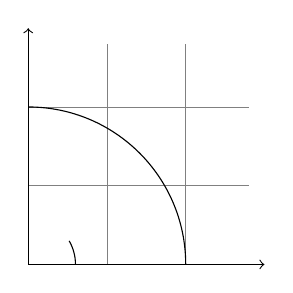
\begin{tikzpicture}[scale=2]
            \draw [step=0.5cm,gray,very thin] (0,0) grid (1.4,1.4);
            \draw [<->] (0,1.5) -- (0,0) -- (1.5,0);
            \draw (1,0) arc (0:90:1cm) (3mm,0pt) arc (0:30:3mm);
        \end{tikzpicture}
    }
    
    \begin{lstlisting}[gobble=8]
        \draw % 0 bis 90 Grad, Radius 1 cm
            (1,0) arc (0:90:1cm)
            % 0 bis 30 Grad, Radius 3 mm
            (3mm,0pt) arc (0:30:3mm);
    \end{lstlisting}
\end{frame}


\begin{frame}[fragile]{Farbig zeichnen}
    \tikzexample{
        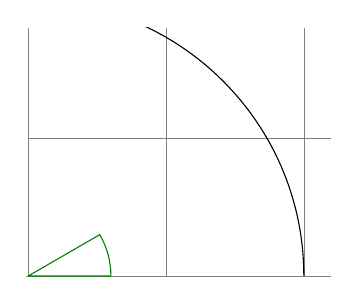
\begin{tikzpicture}[scale=3.5]
            \draw [step=.5cm, very thin, gray] (0,0) grid (1.1,.9);
            \draw [green!50!black] (0,0) -- (3mm,0pt) arc (0:30:3mm) -- cycle;
            
            \clip (0,0) rectangle (1.1,.9);
            \draw (1,0) arc (0:90:1cm);
        \end{tikzpicture}
    }
    
    \begin{lstlisting}[gobble=8]
        \draw [green!50!black]
            (0,0) -- (3mm,0pt) arc (0:30:3mm) -- cycle;
    \end{lstlisting}
\end{frame}


\begin{frame}[fragile]{Farbig füllen}
    \tikzexample{
        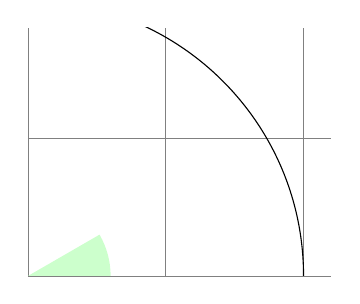
\begin{tikzpicture}[scale=3.5]
            \draw [step=.5cm, very thin, gray] (0,0) grid (1.1,.9);
            \fill [green!20] (0,0) -- (3mm,0pt) arc (0:30:3mm) -- cycle;
            
            \clip (0,0) rectangle (1.1,.9);
            \draw (1,0) arc (0:90:1cm);
        \end{tikzpicture}
    }
    
    \begin{lstlisting}[gobble=8]
        \fill [green!20]
            (0,0) -- (3mm,0pt) arc (0:30:3mm) -- cycle;
    \end{lstlisting}
\end{frame}


\begin{frame}[fragile]{Farbig zeichnen und füllen}
    \tikzexample{
        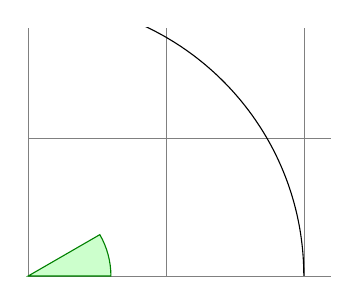
\begin{tikzpicture}[scale=3.5]
            \draw [step=.5cm, very thin, gray] (0,0) grid (1.1,.9);
            \filldraw [fill=green!20,draw=green!50!black] (0,0) -- (3mm,0pt) arc (0:30:3mm) -- cycle;
            
            \clip (0,0) rectangle (1.1,.9);
            \draw (1,0) arc (0:90:1cm);
        \end{tikzpicture}
    }
    
    \begin{lstlisting}[gobble=8]
        \filldraw [fill=green!20,draw=green!50!black]
            (0,0) -- (3mm,0pt) arc (0:30:3mm) -- cycle;
    \end{lstlisting}
\end{frame}


\begin{frame}[fragile]{Polarkoordinaten und Schnittpunkte}
    \tikzexample{
        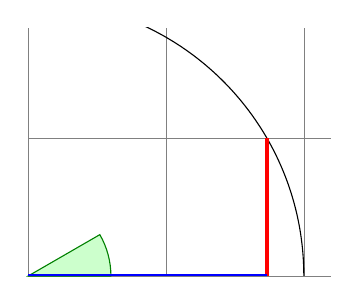
\begin{tikzpicture}[scale=3.5]
            \draw [step=.5cm, very thin, gray] (0,0) grid (1.1,.9);
            \filldraw [fill=green!20,draw=green!50!black] (0,0) -- (3mm,0pt) arc (0:30:3mm) -- cycle;
            
            \clip (0,0) rectangle (1.1,.9);
            \draw (1,0) arc (0:90:1cm);
            
            \draw [very thick, red] (30:1cm) -- (30:1cm |- 0,0);
            \draw [very thick, blue] (0,0) -- (30:1cm |- 0,0);
        \end{tikzpicture}
    }

    \begin{lstlisting}[gobble=12]
            \draw [very thick, red] (30:1cm) -- (30:1cm |- 0,0);
            \draw [very thick, blue] (0,0) -- (30:1cm |- 0,0);
    \end{lstlisting}
\end{frame}


\begin{frame}[fragile]{Schnittpunkte von Pfaden definieren}
    \tikzexample{
        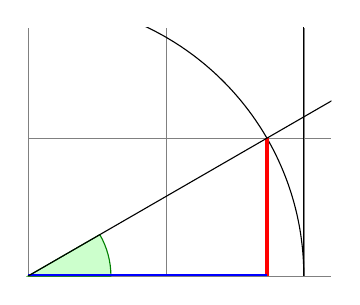
\begin{tikzpicture}[scale=3.5]
            \draw [step=.5cm, very thin, gray] (0,0) grid (1.1,.9);
            \filldraw [fill=green!20,draw=green!50!black] (0,0) -- (3mm,0pt) arc (0:30:3mm) -- cycle;
            
            \clip (0,0) rectangle (1.1,.9);
            \draw (1,0) arc (0:90:1cm);
            
            \draw [very thick, red] (30:1cm) -- (30:1cm |- 0,0);
            \draw [very thick, blue] (0,0) -- (30:1cm |- 0,0);
            
            \draw [name path=l1] (1,0) -- (1,1);
            \draw [name path=l2] (0,0) -- (30:1.5cm);
            \draw [name intersections={of=l1 and l2, by=tan}];
        \end{tikzpicture}
    }

    \begin{lstlisting}[gobble=12]
            \draw [name path=l1] (1,0) -- (1,1);
            \draw [name path=l2] (0,0) -- (30:1.5cm);
            \draw [name intersections={of=l1 and l2, by=tan}];
    \end{lstlisting}
\end{frame}


\begin{frame}[fragile]{Unsichtbare Pfade}
    \tikzexample{
        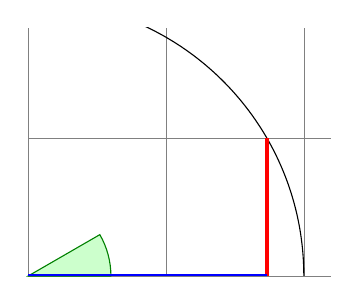
\begin{tikzpicture}[scale=3.5]
            \draw [step=.5cm, very thin, gray] (0,0) grid (1.1,.9);
            \filldraw [fill=green!20,draw=green!50!black] (0,0) -- (3mm,0pt) arc (0:30:3mm) -- cycle;
            
            \clip (0,0) rectangle (1.1,.9);
            \draw (1,0) arc (0:90:1cm);
            
            \draw [very thick, red] (30:1cm) -- (30:1cm |- 0,0);
            \draw [very thick, blue] (0,0) -- (30:1cm |- 0,0);
            
            \path [name path=l1] (1,0) -- (1,1);
            \path [name path=l2] (0,0) -- (30:1.5cm);
            \draw [name intersections={of=l1 and l2, by=tan}];
        \end{tikzpicture}
    }

    \begin{lstlisting}[gobble=12]
            \path [name path=l1] (1,0) -- (1,1);
            \path [name path=l2] (0,0) -- (30:1.5cm);
            \draw [name intersections={of=l1 and l2, by=tan}];
    \end{lstlisting}
\end{frame}


\begin{frame}[fragile]{Schnittpunkte von Pfaden verwenden}
    \tikzexample{
        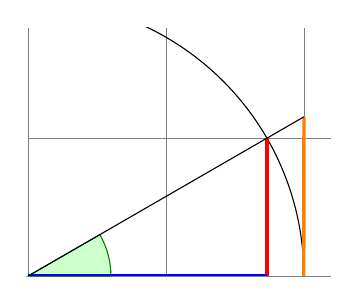
\begin{tikzpicture}[scale=3.5]
            \draw [step=.5cm, very thin, gray] (0,0) grid (1.1,.9);
            \filldraw [fill=green!20,draw=green!50!black] (0,0) -- (3mm,0pt) arc (0:30:3mm) -- cycle;
            
            \clip (0,0) rectangle (1.1,.9);
            \draw (1,0) arc (0:90:1cm);
            
            \draw [very thick, red] (30:1cm) -- (30:1cm |- 0,0);
            \draw [very thick, blue] (0,0) -- (30:1cm |- 0,0);
            
            \path [name path=l1] (1,0) -- (1,1);
            \path [name path=l2] (0,0) -- (30:1.5cm);
            \draw [name intersections={of=l1 and l2, by=tan}];
            
            \draw [very thick, orange] (1,0) -- (tan);
            \draw (0,0) -- (tan);
        \end{tikzpicture}
    }

    \begin{lstlisting}[gobble=12]
            \draw [very thick, orange] (1,0) -- (tan);
            \draw (0,0) -- (tan);
    \end{lstlisting}
\end{frame}


\begin{frame}[fragile]{Beschriftungen}
    \tikzexample{
        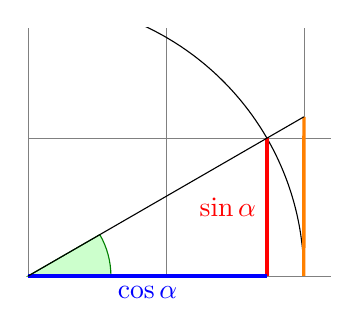
\begin{tikzpicture}[scale=3.5]
            \draw [step=.5cm, very thin, gray] (0,0) grid (1.1,.9);
            \filldraw [fill=green!20,draw=green!50!black] (0,0) -- (3mm,0pt) arc (0:30:3mm) -- cycle;
            
            \clip (0,-.1) rectangle (1.1,.9);
            \draw (1,0) arc (0:90:1cm);
            
            \draw [very thick, red] (30:1cm) -- node [left] {$\sin \alpha$} (30:1cm |- 0,0);
            \draw [very thick, blue] (0,0) -- node [below] {$\cos \alpha$} (30:1cm |- 0,0);
            
            \path [name path=l1] (1,0) -- (1,1);
            \path [name path=l2] (0,0) -- (30:1.5cm);
            \draw [name intersections={of=l1 and l2, by=tan}];
            
            \draw [very thick, orange] (1,0) -- (tan);
            \draw (0,0) -- (tan);
        \end{tikzpicture}
    }

    \begin{lstlisting}[gobble=12]
            \draw [very thick, red] (30:1cm) --
                node [left] {$\sin \alpha$} (30:1cm |- 0,0);
            \draw [very thick, blue] (0,0) --
                node [below] {$\cos \alpha$} (30:1cm |- 0,0);
    \end{lstlisting}
\end{frame}


\begin{frame}[fragile]{Beschriftungen der Achsen}
    \tikzexample{
        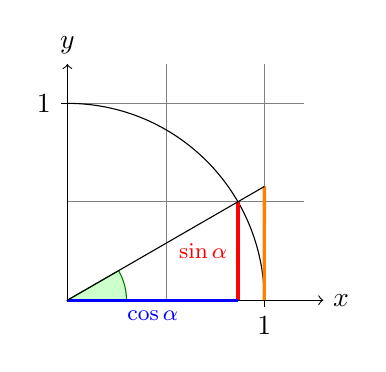
\begin{tikzpicture}[scale=2.5]
            \draw [step=.5cm, very thin, gray] (0,0) grid (1.2,1.2);
            \filldraw [fill=green!20,draw=green!50!black] (0,0) -- (3mm,0pt) arc (0:30:3mm) -- cycle;
            
            \draw[->] (0,0) -- (1.3,0) node[right] {$x$};
            \draw[->] (0,0) -- (0,1.2) node[above] {$y$};
            \draw (1,1pt) -- (1,-1pt) node[below] {$1$};
            \draw (1pt,1) -- (-1pt,1) node[left] {$1$};
            
            %\clip (0,-.1) rectangle (1.1,.9);
            \draw (1,0) arc (0:90:1cm);
            
            \draw [very thick, red] (30:1cm) -- node [left] {\footnotesize$\sin \alpha$} (30:1cm |- 0,0);
            \draw [very thick, blue] (0,0) -- node [below] {\footnotesize$\cos \alpha$} (30:1cm |- 0,0);
            
            \path [name path=l1] (1,0) -- (1,1);
            \path [name path=l2] (0,0) -- (30:1.5cm);
            \draw [name intersections={of=l1 and l2, by=tan}];
            
            \draw [very thick, orange] (1,0) -- (tan);
            \draw (0,0) -- (tan);
        \end{tikzpicture}
    }

    \begin{lstlisting}[gobble=12]
            \draw[->] (0,0) -- (1.5,0) node[right] {$x$};
            \draw[->] (0,0) -- (0,1.5) node[above] {$y$};
            \draw (1,1pt) -- (1,-1pt) node[below] {$1$};
            \draw (1pt,1) -- (-1pt,1) node[left] {$1$};
    \end{lstlisting}
\end{frame}


\section{Graphen}
\subsection{Knoten und Kanten}
\begin{frame}[fragile]{Knoten}
    \begin{columns}
        \begin{column}{.4\textwidth}
            \tikzexample{
                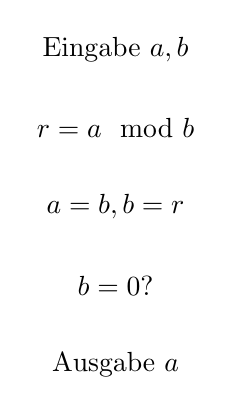
\begin{tikzpicture}
                    \node at (0,4) {Eingabe $a,b$};
                    \node at (0,3) {$r = a \mod b$};
                    \node at (0,2) {$a=b, b=r$};
                    \node at (0,1) {$b=0?$};
                    \node at (0,0) {Ausgabe $a$};
                \end{tikzpicture}
            }  
        \end{column}
        \begin{column}{.6\textwidth}
            \begin{lstlisting}[gobble=12]
                \node at (0,4) {...};
                \node at (0,3) {...};
                \node at (0,2) {...};
                \node at (0,1) {...};
                \node at (0,0) {...};
            \end{lstlisting}
        \end{column}
    \end{columns}
\end{frame}


\begin{frame}[fragile]{Knoten haben Stile}{Ein- und Ausgabe}
    \tikzexample{
        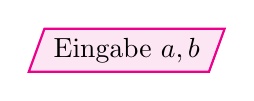
\begin{tikzpicture}
            [io/.style={trapezium,
                trapezium left angle=70,
                trapezium right angle=110,
                fill=magenta!10, draw=magenta}, thick]
            \node[io] {Eingabe $a,b$};
        \end{tikzpicture}
    }
    
    \begin{lstlisting}[gobble=8]
        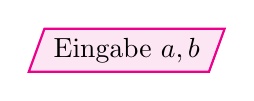
\begin{tikzpicture}
            [io/.style={trapezium,
                trapezium left angle=70,
                trapezium right angle=110,
                fill=magenta!10, draw=magenta}, thick]
            \node[io] {Eingabe $a,b$};
        \end{tikzpicture}
    \end{lstlisting}
\end{frame}


\begin{frame}[fragile]{Knoten haben Stile}{Operationen}
    \tikzexample{
        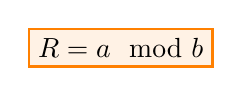
\begin{tikzpicture}
            [op/.style={rectangle,
                fill=orange!10, draw=orange}, thick]
            \node[op] {$R = a \mod b$};
        \end{tikzpicture}
    }
    
    \begin{lstlisting}[gobble=8]
        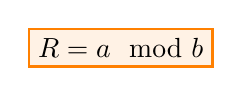
\begin{tikzpicture}
            [op/.style={rectangle,
                fill=orange!10, draw=orange}, thick]
            \node[op] {$R = a \mod b$};
        \end{tikzpicture}
    \end{lstlisting}
\end{frame}


\begin{frame}[fragile]{Knoten haben Stile}{Entscheidungen}
    \tikzexample{
        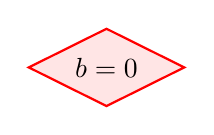
\begin{tikzpicture}
            [cn/.style={diamond,
                aspect=2,
                fill=red!10, draw=red}, thick]
            \node[cn] {$b=0$};
        \end{tikzpicture}
    }
    
    \begin{lstlisting}[gobble=8]
        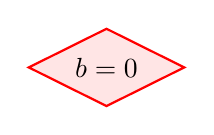
\begin{tikzpicture}
            [cn/.style={diamond,
                aspect=2,
                fill=red!10, draw=red}, thick]
            \node[cn] {$b=0$};
        \end{tikzpicture}
    \end{lstlisting}
\end{frame}


\begin{frame}[fragile]{Knoten haben Namen}
    \begin{columns}
        \begin{column}{.4\textwidth}
            \tikzexample{
                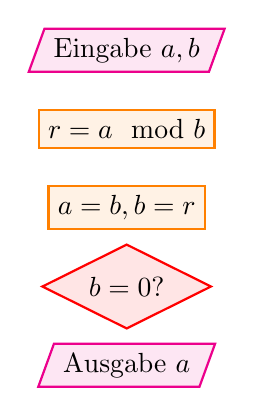
\begin{tikzpicture}
                    [io/.style={trapezium,
                        trapezium left angle=70,
                        trapezium right angle=110,
                        fill=magenta!10, draw=magenta},
                    op/.style={rectangle,
                        fill=orange!10, draw=orange},
                    cn/.style={diamond,
                        aspect=2,
                        fill=red!10, draw=red},
                    thick]
                    
                    \node[io] at (0,4)
                        (in) {Eingabe $a,b$};
                    \node[op] at (0,3)
                        (div) {$r = a \mod b$};
                    \node[op] at (0,2)
                        (set) {$a=b, b=r$};
                    \node[cn] at (0,1)
                        (cond) {$b=0?$};
                    \node[io] at (0,0)
                        (out) {Ausgabe $a$};
                \end{tikzpicture}
            }  
        \end{column}
        \begin{column}{.6\textwidth}
            \begin{lstlisting}[gobble=16]
                \node[io] at (0,4)
                    (in) {Eingabe $a,b$};
                \node[op] at (0,3)
                    (div) {$r = a \mod b$};
                \node[op] at (0,2)
                    (set) {$a=b, b=r$};
                \node[cn] at (0,1)
                    (cond) {$b=0?$};
                \node[io] at (0,0)
                    (out) {Ausgabe $a$};
            \end{lstlisting}
        \end{column}
    \end{columns}
\end{frame}


\begin{frame}[fragile]{Knoten relativ positionieren}
    \begin{columns}
        \begin{column}{.4\textwidth}
            \tikzexample{
                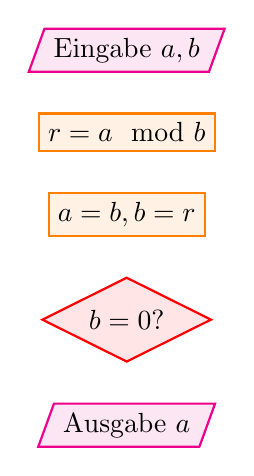
\begin{tikzpicture}
                    [io/.style={trapezium,
                        trapezium left angle=70,
                        trapezium right angle=110,
                        fill=magenta!10, draw=magenta},
                    op/.style={rectangle,
                        fill=orange!10, draw=orange},
                    cn/.style={diamond,
                        aspect=2,
                        fill=red!10, draw=red},
                    thick, node distance=.5cm]
                    
                    \node[io] (in)
                        {Eingabe $a,b$};
                    \node[op, below=of in]
                        (div) {$r = a \mod b$};
                    \node[op, below=of div]
                        (set) {$a=b, b=r$};
                    \node[cn, below=of set]
                        (cond) {$b=0?$};
                    \node[io, below=of cond]
                        (out) {Ausgabe $a$};
                \end{tikzpicture}
            }  
        \end{column}
        \begin{column}{.6\textwidth}
            \begin{lstlisting}[gobble=16]
                \node[io]
                    (in) {Eingabe $a,b$};
                \node[op, below=of in]
                    (div) {$r = a \mod b$};
                \node[op, below=of div]
                    (set) {$a=b, b=r$};
                \node[cn, below=of set]
                    (cond) {$b=0?$};
                \node[io, below=of cond]
                    (out) {Ausgabe $a$};
            \end{lstlisting}
        \end{column}
    \end{columns}
\end{frame}


\begin{frame}[fragile]{Kanten}
    \begin{columns}
        \begin{column}{.4\textwidth}
            \tikzexample{
                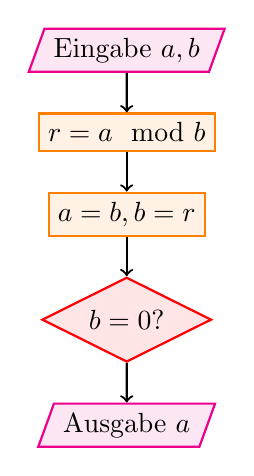
\begin{tikzpicture}
                    [io/.style={trapezium,
                        trapezium left angle=70,
                        trapezium right angle=110,
                        fill=magenta!10, draw=magenta},
                    op/.style={rectangle,
                        fill=orange!10, draw=orange},
                    cn/.style={diamond,
                        aspect=2,
                        fill=red!10, draw=red},
                    thick, node distance=.5cm]
                    
                    \node[io] (in)
                        {Eingabe $a,b$};
                    \node[op, below=of in]
                        (div) {$r = a \mod b$};
                    \node[op, below=of div]
                        (set) {$a=b, b=r$};
                    \node[cn, below=of set]
                        (cond) {$b=0?$};
                    \node[io, below=of cond]
                        (out) {Ausgabe $a$};
                    
                    \path[->]
                        (in)    edge (div)
                        (div)   edge (set)
                        (set)   edge (cond)
                        (cond)  edge (out);
                \end{tikzpicture}
            }  
        \end{column}
        \begin{column}{.6\textwidth}
            \begin{lstlisting}[gobble=16]
                \path[->]
                    (in)    edge (div)
                    (div)   edge (set)
                    (set)   edge (cond)
                    (cond)  edge (out);
            \end{lstlisting}
        \end{column}
    \end{columns}
\end{frame}


\begin{frame}[fragile]{Ein Pfad um die Ecke}
    \begin{columns}
        \begin{column}{.4\textwidth}
            \tikzexample{
                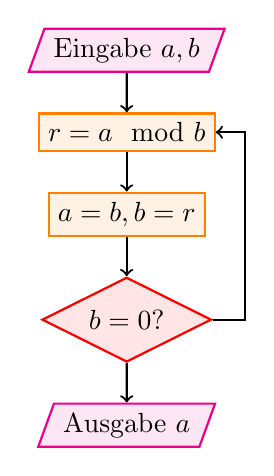
\begin{tikzpicture}
                    [io/.style={trapezium,
                        trapezium left angle=70,
                        trapezium right angle=110,
                        fill=magenta!10, draw=magenta},
                    op/.style={rectangle,
                        fill=orange!10, draw=orange},
                    cn/.style={diamond,
                        aspect=2,
                        fill=red!10, draw=red},
                    thick, node distance=.5cm]
                    
                    \node[io] (in)
                        {Eingabe $a,b$};
                    \node[op, below=of in]
                        (div) {$r = a \mod b$};
                    \node[op, below=of div]
                        (set) {$a=b, b=r$};
                    \node[cn, below=of set]
                        (cond) {$b=0?$};
                    \node[io, below=of cond]
                        (out) {Ausgabe $a$};
                    
                    \path[->]
                        (in)    edge (div)
                        (div)   edge (set)
                        (set)   edge (cond)
                        (cond)  edge (out);
                    
                    \draw[->]
                        (cond)  -- ++ (1.5,0)
                                |- (div);
                \end{tikzpicture}
            }  
        \end{column}
        \begin{column}{.6\textwidth}
            \begin{lstlisting}[gobble=16]
                \draw[->]
                    (cond)  -- ++ (1.5,0)
                            |- (div);
            \end{lstlisting}
        \end{column}
    \end{columns}
\end{frame}


\begin{frame}[fragile]{Ein Pfad um die Ecke}
    \begin{columns}
        \begin{column}{.4\textwidth}
            \tikzexample{
                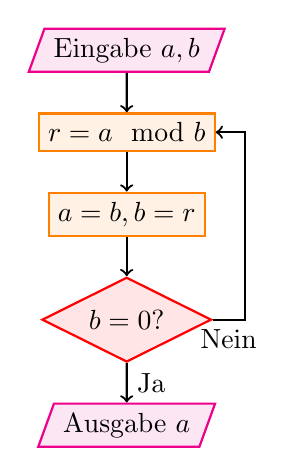
\begin{tikzpicture}
                    [io/.style={trapezium,
                        trapezium left angle=70,
                        trapezium right angle=110,
                        fill=magenta!10, draw=magenta},
                    op/.style={rectangle,
                        fill=orange!10, draw=orange},
                    cn/.style={diamond,
                        aspect=2,
                        fill=red!10, draw=red},
                    thick, node distance=.5cm]
                    
                    \node[io] (in)
                        {Eingabe $a,b$};
                    \node[op, below=of in]
                        (div) {$r = a \mod b$};
                    \node[op, below=of div]
                        (set) {$a=b, b=r$};
                    \node[cn, below=of set]
                        (cond) {$b=0?$};
                    \node[io, below=of cond]
                        (out) {Ausgabe $a$};
                    
                    \path[->]
                        (in)    edge (div)
                        (div)   edge (set)
                        (set)   edge (cond);
                        
                    \path[->]
                        (cond) edge
                            node[right] {Ja}
                                (out);
                    \draw[->]
                        (cond)  --
                            node[below] {Nein}
                                ++ (1.5,0) |- (div);
                \end{tikzpicture}
            }  
        \end{column}
        \begin{column}{.6\textwidth}
            \begin{lstlisting}[gobble=16]
                \path[->]
                    (cond) edge
                        node[right] {Ja}
                            (out);
                
                \draw[->] (cond)  --
                    node[below] {Nein}
                        ++ (1.5,0) |- (div);
            \end{lstlisting}
        \end{column}
    \end{columns}
\end{frame}


\subsection{Automaten}
\begin{frame}[fragile]
    \tikzexample{
        \begin{tikzpicture}
            % Platzhalter
            \draw[draw=red!5] (-2,-1) rectangle (4.5,1.7);
            
            \node[initial, state] (q0) {$q_0$};
        \end{tikzpicture}
    }
    
    \begin{lstlisting}[gobble=8]
        \node[initial, state] (q0) {$q_0$};
        (*@\vphantom{h}@*)
        (*@\vphantom{h}@*)
        (*@\vphantom{h}@*)
        (*@\vphantom{h}@*)
        (*@\vphantom{h}@*)
        (*@\vphantom{h}@*)
        (*@\vphantom{h}@*)
    \end{lstlisting}
\end{frame}


\begin{frame}[fragile]
    \tikzexample{
        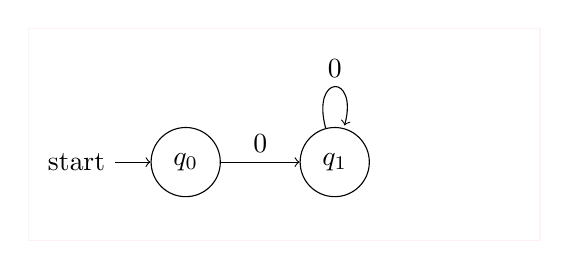
\begin{tikzpicture}
            % Platzhalter
            \draw[draw=red!5] (-2,-1) rectangle (4.5,1.7);
            
            \node[initial, state] (q0) {$q_0$};
            \node[state, right=of q0] (q1) {$q_1$};
            \path    (q0) edge[->] node[above] {0} (q1)
                    (q1) edge[->, loop above] node {0} ();
        \end{tikzpicture}
    }
    
    \begin{lstlisting}[gobble=8]
        \node[initial, state] (q0) {$q_0$};
        \node[state, accepting, right=of q1] (q2) {$q_2$};
        (*@\vphantom{h}@*)
        (*@\vphantom{h}@*)
        \path (q0)    edge[->] node[above] {0} (q1)
              (q1)    edge[->, loop above] node {0} ();
        (*@\vphantom{h}@*)
        (*@\vphantom{h}@*)
    \end{lstlisting}
\end{frame}


\begin{frame}[fragile]
    \tikzexample{
        \begin{tikzpicture}
            % Platzhalter
            \draw[draw=red!5] (-2,-1) rectangle (4.5,1.7);
            
            \node[initial, state] (q0) {$q_0$};
            \node[state, accepting, right=of q1] (q2) {$q_2$};
            \node[state, right=of q0] (q1) {$q_1$};
            \path  (q0)  edge[->] node[above] {0} (q1)
                   (q1)  edge[->, loop above] node {0} ()
                         edge[->, bend left] node[above] {1} (q2)
                   (q2)  edge[->, bend left] node[below] {0} (q1);
        \end{tikzpicture}
    }
    
    \begin{lstlisting}[gobble=8]
        \node[initial, state] (q0) {$q_0$};
        \node[state, accepting, right=of q1] (q2) {$q_2$};
        \node[state, right=of q0] (q1) {$q_1$};
        (*@\vphantom{h}@*)
        \path (q0)    edge[->] node[above] {0} (q1)
              (q1)    edge[->, loop above] node {0} ()
                      edge[->, bend left] node[above] {1} (q2)
              (q2)    edge[->, bend left] node[below] {0} (q1);
    \end{lstlisting}
\end{frame}


\subsection{Bäume}
\begin{frame}[fragile]
    \begin{columns}
        \begin{column}{.45\textwidth}
            \tikzexample{
                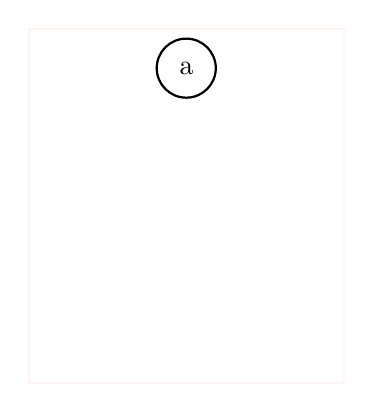
\begin{tikzpicture}
                    [
                        every node/.style={draw,circle,thick, minimum size=.75cm},
                        every path/.style={thick},
                        level 1/.style={sibling distance=2cm},
                        level 2/.style={sibling distance=1cm}
                    ]
                    
                    % Platzhalter
                    \draw[draw=red!5] (-2,.5) rectangle (2,-4);
                    
                    \node {a};
                \end{tikzpicture}
            }
        \end{column}
        \begin{column}{.55\textwidth}
            \begin{lstlisting}[gobble=16]
                \node {a};
                (*@\vphantom{h}@*)
                (*@\vphantom{h}@*)
                (*@\vphantom{h}@*)
                (*@\vphantom{h}@*)
                (*@\vphantom{h}@*)
                (*@\vphantom{h}@*)
                (*@\vphantom{h}@*)
                (*@\vphantom{h}@*)
            \end{lstlisting}
        \end{column}
    \end{columns}
\end{frame}


\begin{frame}[fragile]
    \begin{columns}
        \begin{column}{.45\textwidth}
            \tikzexample{
                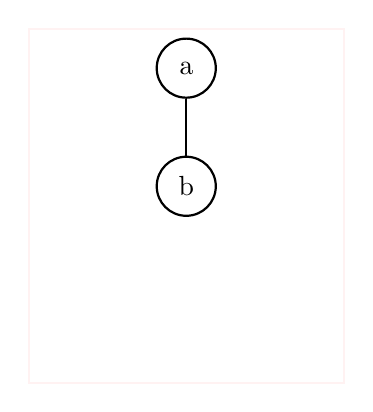
\begin{tikzpicture}
                    [
                        every node/.style={draw,circle,thick, minimum size=.75cm},
                        every path/.style={thick},
                        level 1/.style={sibling distance=2cm},
                        level 2/.style={sibling distance=1cm}
                    ]
                    
                    % Platzhalter
                    \draw[draw=red!5] (-2,.5) rectangle (2,-4);
                    
                    \node {a}
                        child { node {b} };
                \end{tikzpicture}
            }
        \end{column}
        \begin{column}{.55\textwidth}
            \begin{lstlisting}[gobble=16]
                \node {a}
                    child { node {b} };
                (*@\vphantom{h}@*)
                (*@\vphantom{h}@*)
                (*@\vphantom{h}@*)
                (*@\vphantom{h}@*)
                (*@\vphantom{h}@*)
                (*@\vphantom{h}@*)
                (*@\vphantom{h}@*)
            \end{lstlisting}
        \end{column}
    \end{columns}
\end{frame}


\begin{frame}[fragile]
    \begin{columns}
        \begin{column}{.45\textwidth}
            \tikzexample{
                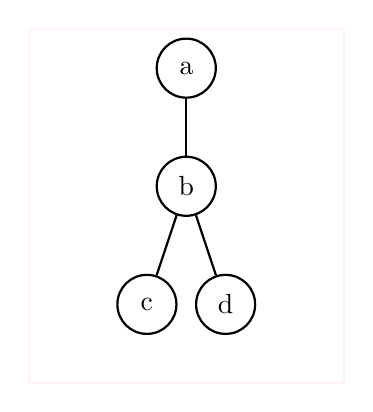
\begin{tikzpicture}
                    [
                        every node/.style={draw,circle,thick, minimum size=.75cm},
                        every path/.style={thick},
                        level 1/.style={sibling distance=2cm},
                        level 2/.style={sibling distance=1cm}
                    ]
                    
                    % Platzhalter
                    \draw[draw=red!5] (-2,.5) rectangle (2,-4);
                    
                    \node {a}
                        child { node {b}
                            child { node {c} }
                            child { node {d} }
                        };
                \end{tikzpicture}
            }
        \end{column}
        \begin{column}{.55\textwidth}
            \begin{lstlisting}[gobble=16]
                \node {a}
                    child { node {b}
                        child { node {c} }
                        child { node {d} }
                    };
                (*@\vphantom{h}@*)
                (*@\vphantom{h}@*)
                (*@\vphantom{h}@*)
                (*@\vphantom{h}@*)
            \end{lstlisting}
        \end{column}
    \end{columns}
\end{frame}


\begin{frame}[fragile]
    \begin{columns}
        \begin{column}{.45\textwidth}
            \tikzexample{
                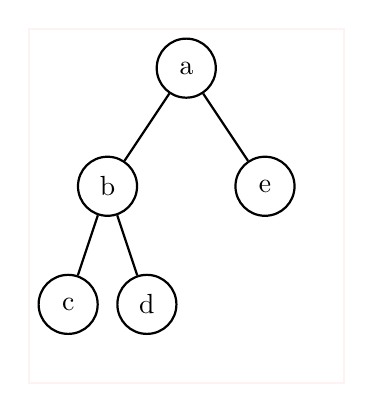
\begin{tikzpicture}
                    [
                        every node/.style={draw,circle,thick, minimum size=.75cm},
                        every path/.style={thick},
                        level 1/.style={sibling distance=2cm},
                        level 2/.style={sibling distance=1cm}
                    ]
                    
                    % Platzhalter
                    \draw[draw=red!5] (-2,.5) rectangle (2,-4);
                    
                    \node {a}
                        child { node {b}
                            child { node {c} }
                            child { node {d} }
                        }
                        child { node {e} };
                \end{tikzpicture}
            }
        \end{column}
        \begin{column}{.55\textwidth}
            \begin{lstlisting}[gobble=16]
                \node {a}
                    child { node {b}
                        child { node {c} }
                        child { node {d} }
                    }
                    child { node {e} };
                (*@\vphantom{h}@*)
                (*@\vphantom{h}@*)
                (*@\vphantom{h}@*)
            \end{lstlisting}
        \end{column}
    \end{columns}
\end{frame}


\begin{frame}[fragile]
    \begin{columns}
        \begin{column}{.45\textwidth}
            \tikzexample{
                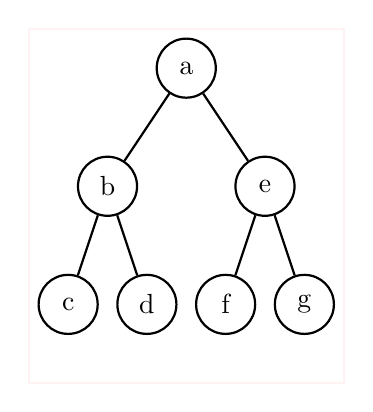
\begin{tikzpicture}
                    [
                        every node/.style={draw,circle,thick, minimum size=.75cm},
                        every path/.style={thick},
                        level 1/.style={sibling distance=2cm},
                        level 2/.style={sibling distance=1cm}
                    ]
                    
                    % Platzhalter
                    \draw[draw=red!5] (-2,.5) rectangle (2,-4);
                    
                    \node {a}
                        child { node {b}
                            child { node {c} }
                            child { node {d} }
                        }
                        child { node {e}
                            child { node {f} }
                            child { node {g} }
                        };
                \end{tikzpicture}
            }
        \end{column}
        \begin{column}{.55\textwidth}
            \begin{lstlisting}[gobble=16]
                \node {a}
                    child { node {b}
                        child { node {c} }
                        child { node {d} }
                    }
                    child { node {e}
                        child { node {f} }
                        child { node {g} }
                    };
            \end{lstlisting}
        \end{column}
    \end{columns}
\end{frame}


\section{Fortgeschrittene Verwendung}
\subsection{Funktionen plotten}
\begin{frame}{Beispiel eines Funktionsplots}
    \tikzexample{
        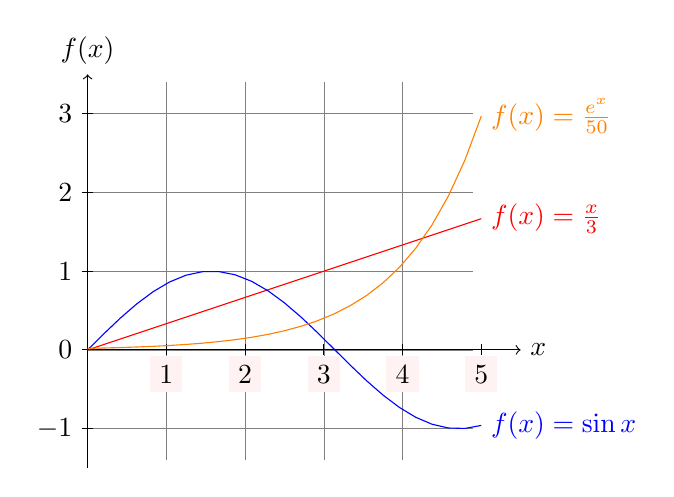
\begin{tikzpicture}
            []
            
            \draw[very thin,gray] (0,-1.4) grid (4.9,3.4);
            
            \draw[->] (0,-1.5) -- (0,3.5) node[above] {$f(x)$};
            \foreach \y in {-1,...,3} {
                \draw (2pt,\y) -- ++ (-4pt,0) node[left] {$\y$};
            }
            \draw[->] (0,0) -- (5.5,0) node[right] {$x$};
            \foreach \x in {1,...,5} {
                \draw (\x,2pt) -- ++ (0,-4pt) node[below,fill=red!5] {$\x$};
            }
            
            \draw[domain=0:5,red] plot (\x,\x/3) node[right] {$f(x) = \frac{x}{3}$};
            \draw[domain=0:5,blue] plot (\x,{sin(\x r)}) node[right] {$f(x) = \sin x$};
            \draw[domain=0:5,orange] plot (\x,{exp(\x)/50}) node[right] {$f(x) = \frac{e^x}{50}$};
        \end{tikzpicture}
    }
\end{frame}

\begin{frame}[fragile]
    \tikzexample{
        \begin{tikzpicture}
            \draw[blue,domain=0:5] plot (\x,{sin(\x r)});
            \draw[orange,domain=0:4] plot (\x,{exp(\x)/50});
        \end{tikzpicture}
    }
    
    \begin{lstlisting}[gobble=8]
        \draw[blue,domain=0:5] plot (\x,{sin(\x r)});
        \draw[orange,domain=0:4] plot (\x,{exp(\x)/50});
    \end{lstlisting}
\end{frame}

\begin{frame}[fragile]{Koordinatensystem}
    \tikzexample{
        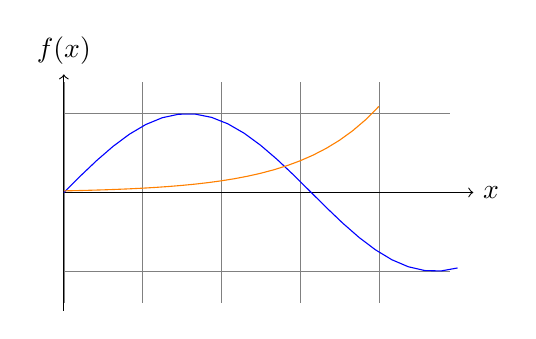
\begin{tikzpicture}
            \draw[very thin,gray] (0,-1.4) grid (4.9,1.4);
            \draw[->] (0,0) -- (5.2,0) node[right] {$x$};
            \draw[->] (0,-1.5) -- (0,1.5) node[above] {$f(x)$};
        
            \draw[blue,domain=0:5] plot (\x,{sin(\x r)});
            \draw[orange,domain=0:4] plot (\x,{exp(\x)/50});
        \end{tikzpicture}
    }
    
    \begin{lstlisting}[gobble=8]
        \draw[very thin,gray] (0,-1.4) grid (4.9,1.4);
        \draw[->] (0,0) -- (5.2,0) node[right] {$x$};
        \draw[->] (0,-1.5) -- (0,1.5) node[above] {$f(x)$};
    \end{lstlisting}
\end{frame}

\begin{frame}[fragile]{Beschriftung der Achsen}
    \tikzexample{
        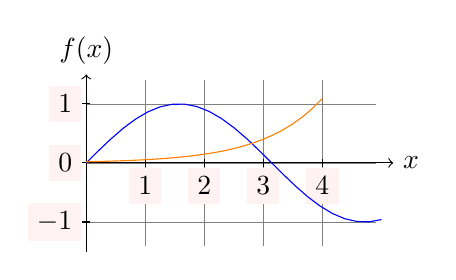
\begin{tikzpicture}
            [
                scale=.75
            ]
            
            \draw[very thin,gray] (0,-1.4) grid (4.9,1.4);
            \draw[->] (0,0) -- (5.2,0) node[right] {$x$};
            \draw[->] (0,-1.5) -- (0,1.5) node[above] {$f(x)$};
            
            \foreach \x in {1,...,4}
                \draw (\x cm,2pt) -- (\x cm,-2pt)
                    node[below,fill=red!5] {$\x$};
            \foreach \y in {-1,...,1}
                \draw (2pt,\y cm) -- (-2pt,\y cm)
                    node[left,fill=red!5] {$\y$};
        
            \draw[blue,domain=0:5] plot (\x,{sin(\x r)});
            \draw[orange,domain=0:4] plot (\x,{exp(\x)/50});
        \end{tikzpicture}
    }
    
    \begin{lstlisting}[gobble=8]
        \foreach \x in {1,...,4}
            \draw (\x cm,2pt) -- (\x cm,-2pt)
                node[below,fill=white] {$\x$};
        \foreach \y in {-1,...,1}
            \draw (2pt,\y cm) -- (-2pt,\y cm)
                node[left,fill=white] {$\y$};
    \end{lstlisting}
\end{frame}

\begin{frame}[fragile]{Beschriftung der Graphen}
    \tikzexample{
        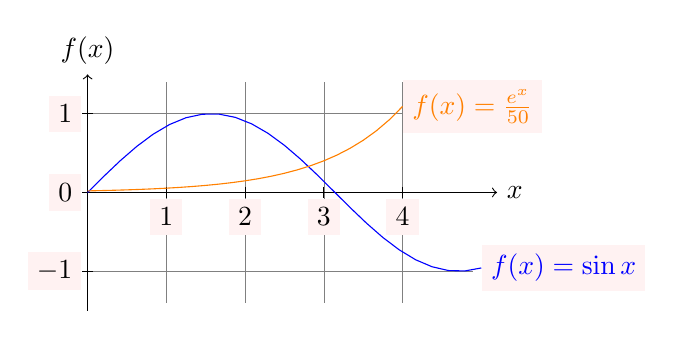
\begin{tikzpicture}
            \draw[very thin,gray] (0,-1.4) grid (4.9,1.4);
            \draw[->] (0,0) -- (5.2,0) node[right] {$x$};
            \draw[->] (0,-1.5) -- (0,1.5) node[above] {$f(x)$};
            
            \foreach \x in {1,...,4}
                \draw (\x cm,2pt) -- (\x cm,-2pt)
                    node[below,fill=red!5] {$\x$};
            \foreach \y in {-1,...,1}
                \draw (2pt,\y cm) -- (-2pt,\y cm)
                    node[left,fill=red!5] {$\y$};
        
            \draw[blue,domain=0:5] plot (\x,{sin(\x r)}) node[right,fill=red!5] {$f(x) = \sin x$};
            \draw[orange,domain=0:4] plot (\x,{exp(\x)/50}) node[right,fill=red!5] {$f(x) = \frac{e^x}{50}$};
        \end{tikzpicture}
    }
    
    \begin{lstlisting}[gobble=8]
        \draw[blue,domain=0:5] plot (\x,{sin(\x r)})
            node[right,fill=white] {$f(x) = \sin x$};
        \draw[orange,domain=0:4] plot (\x,{exp(\x)/50})
            node[right,fill=white] {$f(x) = \frac{e^x}{50}$};
    \end{lstlisting}
\end{frame}


\subsection{Weitere Beispiele}
\begin{frame}[shrink]{Computer science mindmap}{Autor: Till Tantau}
        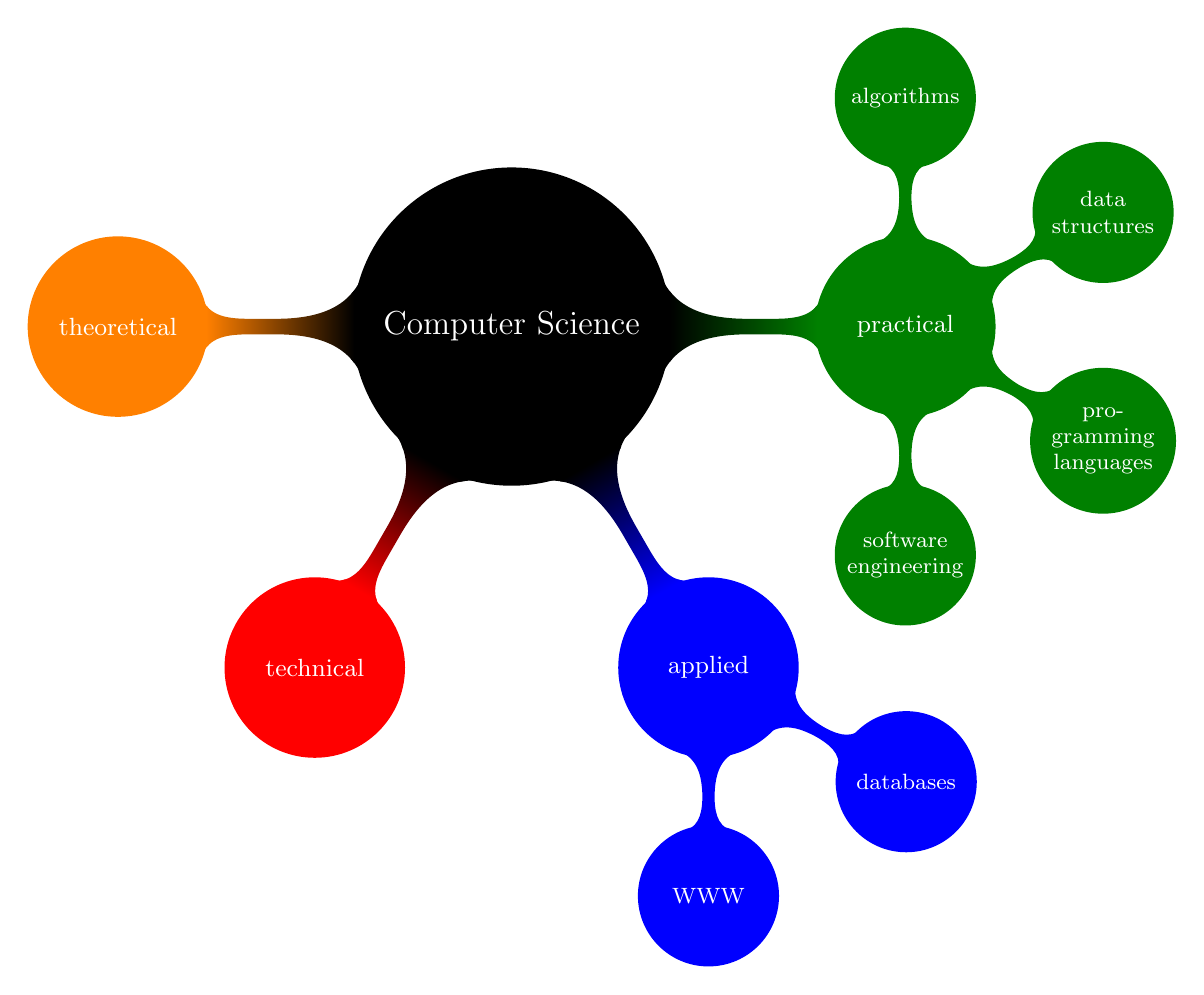
\begin{tikzpicture}
        \path[mindmap,concept color=black,text=white]
    node[concept] {Computer Science}
    [clockwise from=0]
    child[concept color=green!50!black] {
      node[concept] {practical}
      [clockwise from=90]
      child { node[concept] {algorithms} }
      child { node[concept] {data structures} }
      child { node[concept] {pro\-gramming languages} }
      child { node[concept] {software engineer\-ing} }
    }  
    child[concept color=blue] {
      node[concept] {applied}
      [clockwise from=-30]
      child { node[concept] {databases} }
      child { node[concept] {WWW} }
    }
    child[concept color=red] { node[concept] {technical} }
    child[concept color=orange] { node[concept] {theoretical} };
\end{tikzpicture}
\end{frame}

\begin{frame}{A family tree}{Autor: Stefan Kottwitz}
    \begin{tikzpicture}[
  man/.style={rectangle,draw,fill=blue!20},
  woman/.style={rectangle,draw,fill=red!20,rounded corners=.8ex},
  grandchild/.style={grow=down,xshift=1em,anchor=west,
    edge from parent path={(\tikzparentnode.south) |- (\tikzchildnode.west)}},
  first/.style={level distance=6ex},
  second/.style={level distance=12ex},
  third/.style={level distance=18ex},
  level 1/.style={sibling distance=5em}]
    % Parents
    \coordinate
      child[grow=left] {node[man,anchor=east]{Jim}}
      child[grow=right] {node[woman,anchor=west]{Jane}}
      child[grow=down,level distance=0ex]
    [edge from parent fork down]
    % Children and grandchildren
    child{node[man] {Alfred}
      child[grandchild,first] {node[man]{Joe}}
      child[grandchild,second] {node[woman]{Heather}}
      child[grandchild,third] {node[woman] {Barbara}}}
    child{node[woman] {Berta}
      child[grandchild,first] {node[man]{Howard}}}
    child {node[man] {Charles}}
    child {node[woman]{Doris}
      child[grandchild,first] {node[man]{Nick}}
      child[grandchild,second] {node[woman]{Liz}}};
\end{tikzpicture}
\end{frame}

\begin{frame}[shrink]{Christmas tree with balls, candles and snowflakes}{Autor: Alain Matthes}
      \begin{tikzpicture}[  ball red/.style={
    decorate,
    decoration={
      markings,
      mark=between positions .2 and 1 step 3cm
      with
      {
        \pgfmathsetmacro{\sz}{2 + .5 * rand}
        \path[shading=ball,ball color=red] (0,0) circle[radius=\sz mm];
      }
    }
  } ,ball blue/.style={
    decorate,
    decoration={
      markings,
      mark=between positions 0.1 and .9 step 3cm
      with
      {
        \pgfmathsetmacro{\sz}{2 + .5 * rand}
        \path[shading=ball,ball color=blue] (0,0) circle[radius=\sz mm];
      }
    }
  }   
]

\draw[fill=Maroon,ultra thick] 
      (.75,-1)  ..  controls (.5,.5)  and   (.5,3)    .. (0.5,4) 
   -- (-0.5,4)  ..  controls (-.5,3) and (-.5,.5)     .. (-.75,-1) ;
\draw[ultra thick,fill=green!50!black] 
      (0,10) .. controls  (0,8)     and   (1,7)    .. (1.5,7) 
             ..  controls (1,7)     and   (1,7)    .. (0.5,7.25) 
             ..  controls (1.5,5)   and   (2.5,4)  .. (3,4)
             ..  controls (2,4)     and   (1.25,4) .. (1,4.5)
             ..  controls (2,2)     and   (3.5,2)  .. (4,2)
             ..  controls (1,1)     and   (-1,1)   .. (-4,2) 
             ..  controls (-3.5,2)  and   (-2,2)   .. (-1,4.5)
             ..  controls (-1.25,4) and   (-2,4)   .. (-3,4) 
             ..  controls (-2.5,4)  and   (-1.5,5) .. (-0.5,7.25) 
             ..  controls  (-1,7)   and   (-1,7)   .. (-1.5,7)
             ..  controls  (-1,7)   and   (0,8)    .. (0,10)
              ;

\foreach \candle in {(2,5),(-2,5),(0.5,7.5),(-0.5,7.5),(-3,2.5), (3,2.5),
                    (1.5,1.75),(-1.5,1.75)}
\node at \candle {\usebox{\mycandle}} ; 
\node [star, star point height=.5cm, minimum size=.5cm,draw,fill=yellow,thick]
      at (0,10) {};
\begin{scope}[decoration={shape sep=.2cm, shape size=.25cm}] 
    \draw [my star=6, paint=red]  (-4,2)
             ..  controls (0,2)     and   (1,3.5)   .. (1,4.40); 
    \draw [my star=6, paint=red]  (-1.5,5.40)
             ..  controls (0,5.40)     and   (0.5,6.5)      .. (0.5,7);  
    \draw [my star=6, paint=blue]  (4,2)
             ..  controls  (0,2) and (-1,3.5)      .. (-1,4.40);             
    \draw [my star=6, paint=blue]  (1.5,5.40)
             ..  controls (0,5.40)     and   (-0.5,6.5)      .. (-0.5,7);     
\end{scope} 
% the balls
\path[ball red] 
      (0,10) .. controls  (0,8)     and   (1,7)    .. (1.5,7) 
             ..  controls (1,7)     and   (1,7)    .. (0.5,7.25) 
             ..  controls (1.5,5)   and   (2.5,4)  .. (3,4)
             ..  controls (2,4)     and   (1.25,4) .. (1,4.5)
             ..  controls (2,2)     and   (3.5,2)  .. (4,2)
             ..  controls (1,1)     and   (-1,1)   .. (-4,2) 
             ..  controls (-3.5,2)  and   (-2,2)   .. (-1,4.5)
             ..  controls (-1.25,4) and   (-2,4)   .. (-3,4) 
             ..  controls (-2.5,4)  and   (-1.5,5) .. (-0.5,7.25) 
             ..  controls  (-1,7)   and   (-1,7)   .. (-1.5,7)
             ..  controls  (-1,7)   and   (0,8)    .. (0,10)
              ; 
\path[ball blue] 
      (0,10) .. controls  (0,8)     and   (1,7)    .. (1.5,7) 
             ..  controls (1,7)     and   (1,7)    .. (0.5,7.25) 
             ..  controls (1.5,5)   and   (2.5,4)  .. (3,4)
             ..  controls (2,4)     and   (1.25,4) .. (1,4.5)
             ..  controls (2,2)     and   (3.5,2)  .. (4,2)
             ..  controls (1,1)     and   (-1,1)   .. (-4,2) 
             ..  controls (-3.5,2)  and   (-2,2)   .. (-1,4.5)
             ..  controls (-1.25,4) and   (-2,4)   .. (-3,4) 
             ..  controls (-2.5,4)  and   (-1.5,5) .. (-0.5,7.25) 
             ..  controls  (-1,7)   and   (-1,7)   .. (-1.5,7)
             ..  controls  (-1,7)   and   (0,8)    .. (0,10)
              ; 
 % the snow
\foreach \i in {0.5,0.6,...,1.6}
     \fill [white!80!blue,decoration=Koch snowflake,opacity=.9]
           [shift={(rand*5,rnd*8)},scale=\i]
           [double copy shadow={opacity=0.2,shadow xshift=0pt,
           shadow yshift=3*\i pt,fill=white,draw=none}]
        decorate {
          decorate {
            decorate {
              (0,0) -- ++(60:1) -- ++(-60:1) -- cycle
            }
          }
        };                  
\end{tikzpicture}
\end{frame}

\begin{frame}[shrink]{Membrane-like surface}{Autor: Yotam Avital}
  \begin{tikzpicture}[scale=0.8]
    \def\nuPi{3.1459265}
    \foreach \i in {11,10,...,0}{% This one doesn't matter
      \foreach \j in {5,4,...,0}{% This will crate a membrane
                                 % with the front lipids visible
        % top layer
        \pgfmathsetmacro{\dx}{rand*0.1}% A random variance in the x coordinate
        \pgfmathsetmacro{\dy}{rand*0.1}% A random variance in the y coordinate,
                                       % gives a hight fill to the lipid
        \pgfmathsetmacro{\rot}{rand*0.1}% A random variance in the
                                        % molecule orientation
        \shade[ball color=red] ({\i+\dx+\rot},{0.5*\j+\dy+0.4*sin(\i*\nuPi*10)}) circle(0.45);
        \shade[ball color=gray] (\i+\dx,{0.5*\j+\dy+0.4*sin(\i*\nuPi*10)-0.9}) circle(0.45);
        \shade[ball color=gray] (\i+\dx-\rot,{0.5*\j+\dy+0.4*sin(\i*\nuPi*10)-1.8}) circle(0.45);
        % bottom layer
        \pgfmathsetmacro{\dx}{rand*0.1}
        \pgfmathsetmacro{\dy}{rand*0.1}
        \pgfmathsetmacro{\rot}{rand*0.1}
        \shade[ball color=gray] (\i+\dx+\rot,{0.5*\j+\dy+0.4*sin(\i*\nuPi*10)-2.8}) circle(0.45);
        \shade[ball color=gray] (\i+\dx,{0.5*\j+\dy+0.4*sin(\i*\nuPi*10)-3.7}) circle(0.45);
        \shade[ball color=red] (\i+\dx-\rot,{0.5*\j+\dy+0.4*sin(\i*\nuPi*10)-4.6}) circle(0.45);
      }
    }
  \end{tikzpicture}
\end{frame}


\section{Zusammenfassung}
\begin{frame}{Zusammenfassung}
  \begin{enumerate}
    \item TikZ-Zeichnungen bestehen aus \alert{Pfaden}, die über \alert{Koordinaten} definiert werden.
    \item Fast alle scheamtischen Zeichnungen sind ein \alert{Graph}, bestehen also aus \alert{Knoten} und \alert{Kanten} und
      werden auch als solche in TikZ gezeichnet.
    \item TikZ ist sehr umfangreich und enthält \alert{sehr viele Bibliotheken}.
    \item Bei Problemen und Fragen \alert{lies die Anleitung!}
  \end{enumerate}
\end{frame}

\begin{frame}{Zum Weiterlesen}
  \begin{mybib}
    \bibitem{Tantau4}
      Till Tantau.
      \newblock \emph{The TikZ and pgf Packages},
      \newblock Manual for version 2.10,
      \newblock \alt<presentation>{\href{http://www.texample.net/media/pgf/builds/pgfmanualCVS2012-11-04.pdf}{\texttt{pgfmanual.pdf}}}{\url{http://www.texample.net/media/pgf/builds/pgfmanualCVS2012-11-04.pdf}}, November 2012.

    \bibitem{Texample}
      Kjell Magne Fauske und Stefan Kottwitz.
      \newblock \emph{\TeX ample.net},
      \newblock Sample resources for TeX users,
      \newblock \alt<presentation>{\href{http://www.texample.net/tikz/examples/}{\texttt{texample.net}}}{\url{http://www.texample.net/tikz/examples/}}.
  \end{mybib}
\end{frame}

\begin{frame}{GitHub -- Links}
\begin{itemize}
    \item Meine Dateien: \newline 
    \url{https://github.com/labitzkedennis/Nook2016-TikZ}
    \item \LaTeX{} - Präsentationen mit Beamer von Anika Oellerich \newline
    \url{https://github.com/anioell/Nook-LaTeX-Beamer}
    \item Einführung in \LaTeX{} von Malte Schmitz\newline
    \url{https://github.com/malteschmitz/latex}
\end{itemize}
\end{frame}

\end{document}
